\documentclass{article}
\usepackage{graphicx}
\title{Heat Power vs. Inner Core Temperature}
\author{Jin Liu}
\setlength\parindent{0pt}
\begin{document}
\maketitle


The study of the heat power vs. the inner core temperature without Q-pulse.\\
Table 1. lists the files of the sequence and log files for this report.

\begin{table}
[h]
\centering
\caption{Files Name}
\begin{tabular}{|c|c|}
\hline
Sequence & He100to600CtempOnly100sccm\.csv\\ \hline
Log 1 & CONF00/2016-07-21/B37\_day\_21.csv\\  \hline
Log 2 & CONF00/2016-07-21/B37\_day\_21.csv\\ \hline
\end{tabular}
\end{table}


The Inner Core Temperature and Heat Power vs. running hours see Figure 1. 
The Heat Power vs. Inner Core Temperature with the fitted quadratic equation see Figure 2 and Figure 3. 


\begin{figure}
[h]
\begin{center}
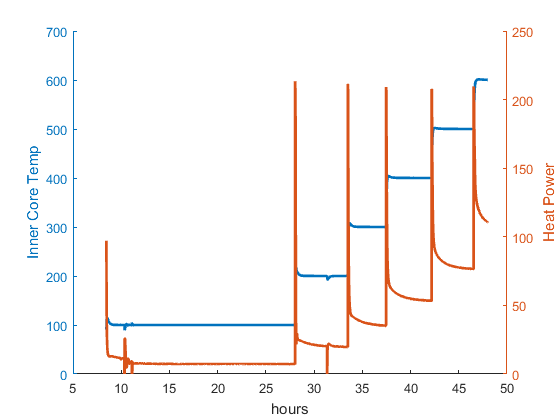
\includegraphics[scale=0.7]{hourvsTempPower.png} 
\caption{Inner Core Temperature and Heat Power vs. Running Hours}%
\end{center}
\end{figure}

\begin{figure}
[h]
\begin{center}
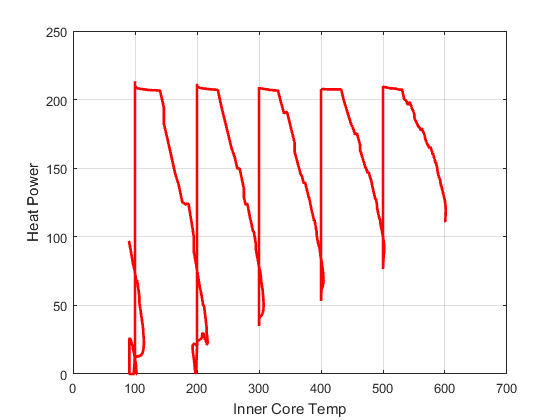
\includegraphics[scale=0.7]{tempvspower.png} 
\caption{Heat Power vs Inner Core Temperature}%
\end{center}
\end{figure}
\begin{figure}
[h]
\begin{center}
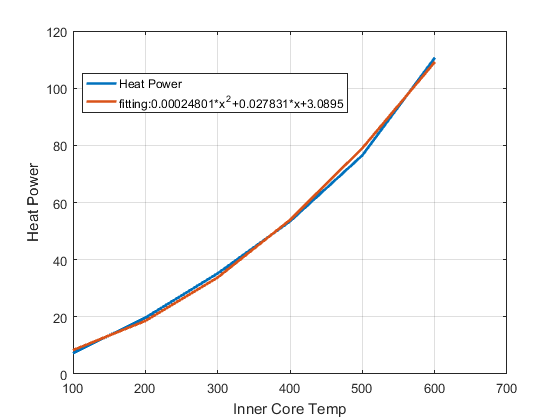
\includegraphics[scale=0.7]{08132016heattemp.png} 
\caption{Heat Power vs Inner Core Temperature with Fitting Curve}%
\end{center}
\end{figure}
\end{document}
